The following example shows how to run the simulation in a simulation loop. This is important if we want to couple the model and implement feedbacks, or as in this case, if we want to retrieve information over time. The following script shows how to calculate the organ lengths over time. 

\lstinputlisting[language=Python, caption=Organ development over time]{examples/topics_development.py}

\begin{itemize}
\item[8-13] Sets up the simulation.

\item[15-17] Defines the simulation time, time step, and the resulting number of simulate(dt) calls. 

\item[23-36] The simulation loop executes the simulation for a single time step L26. After each simulation step, we retrieve the organ type, the sub type, and the length of each organ (L28-30). It is possible to access all root random parameters and resulting realisations using plant.getParameter. In C++ the class functions are defined in Plant::getParameter, Organ::getParameter. In L31-36 we sum up specific organ lengths by boolean array indexing.

\item[38-47] Creates Figure \ref{fig:topics_development}.

\end{itemize}


Next we show how retrieve root tip and root base positions from a simulation. Each organ is represented by a polyline, which is a list of points connected by segments. We use this polyline to plot the base (first node of the polyline) and the tip (last node of the polyline). 

\lstinputlisting[language=Python, caption=Organ tips and bases over time]{examples/topics_development2.py}

\begin{itemize}

\item[8-17] Sets up the simulation and simulation loop as before.

\item[21-28] L23 performs the simulation for a single time step. First we retrieve all organs as polylines L25, where organ tips are the last nodes of the polylines L27, and organ bases are the first nodes L28. Organs that have not started to emerge have only 1 node, and are not retrieved by getPolylines().

\item[30,31] Convert the lists to numpy array for indexing.

\item[33-41] Creates Figure \ref{fig:topics_development2}. In CPlantBox roots are growing with a negative exponential growth rate, i.e. growth becomes slower towards the root reaching its maximal length. Therefore, the node density becomes higher towards the root tips. 

\end{itemize}

\begin{figure}
\begin{subfigure}[c]{0.5\textwidth}
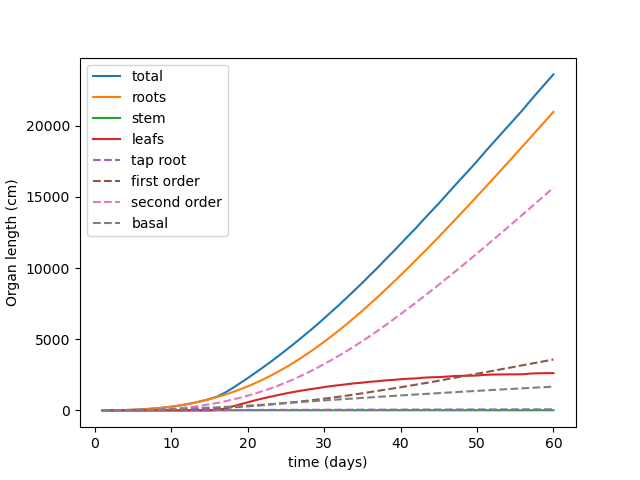
\includegraphics[width=0.99\textwidth]{examples/results/topics_development.png}
\subcaption{Total organ lengths versus time} \label{fig:topics_development}
\end{subfigure}
\begin{subfigure}[c]{0.5\textwidth}
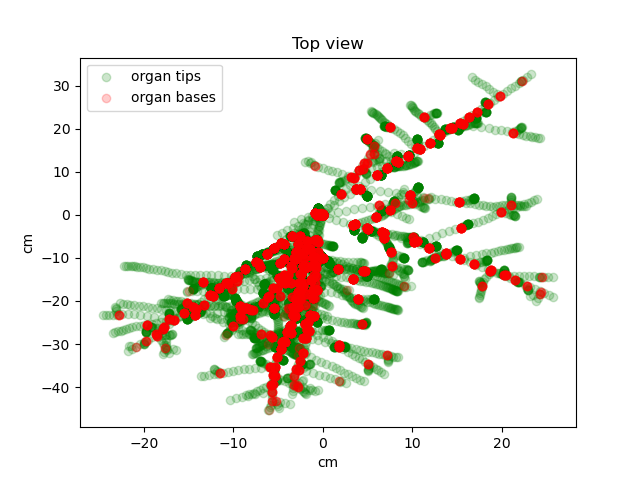
\includegraphics[width=0.99\textwidth]{examples/results/topics_development2.png}
\subcaption{Top view of the organ tip and bases} \label{fig:topics_development2}
\end{subfigure}
\caption{Plant development over time} 
\end{figure}


